% Template for Cogsci submission with R Markdown

% Stuff changed from original Markdown PLOS Template
\documentclass[10pt, letterpaper]{article}

\usepackage{cogsci}
\usepackage{pslatex}
\usepackage{float}
\usepackage{caption}

% amsmath package, useful for mathematical formulas
\usepackage{amsmath}

% amssymb package, useful for mathematical symbols
\usepackage{amssymb}

% hyperref package, useful for hyperlinks
\usepackage{hyperref}

% graphicx package, useful for including eps and pdf graphics
% include graphics with the command \includegraphics
\usepackage{graphicx}

% Sweave(-like)
\usepackage{fancyvrb}
\DefineVerbatimEnvironment{Sinput}{Verbatim}{fontshape=sl}
\DefineVerbatimEnvironment{Soutput}{Verbatim}{}
\DefineVerbatimEnvironment{Scode}{Verbatim}{fontshape=sl}
\newenvironment{Schunk}{}{}
\DefineVerbatimEnvironment{Code}{Verbatim}{}
\DefineVerbatimEnvironment{CodeInput}{Verbatim}{fontshape=sl}
\DefineVerbatimEnvironment{CodeOutput}{Verbatim}{}
\newenvironment{CodeChunk}{}{}

% cite package, to clean up citations in the main text. Do not remove.
\usepackage{cite}

\usepackage{color}

% Use doublespacing - comment out for single spacing
%\usepackage{setspace}
%\doublespacing


% % Text layout
% \topmargin 0.0cm
% \oddsidemargin 0.5cm
% \evensidemargin 0.5cm
% \textwidth 16cm
% \textheight 21cm

\title{Conceptual and prosodic cues in child-directed speech can help children
learn the meaning of disjunction}


\author{{\large \bf Masoud Jasbi} \\ \texttt{masoudj@stanford.edu} \\ Department of Linguistics \\ Stanford University \And {\large \bf Akshay Jaggi} \\ \texttt{ajaggi@stanford.edu} \\ Department of Linguistics \\ Stanford University \And {\large \bf Michael C. Frank} \\ \texttt{mcfrank@stanford.edu} \\ Department of Psychology \\ Stanford University }

\begin{document}

\maketitle

\begin{abstract}
At first glance, children's word learning appears to be mostly a problem
of learning words like \emph{dog} and \emph{run}. However, it is small
words like \emph{and} and \emph{or} that enable the construction of
complex combinatorial language. How do children learn the meaning of
these function words? Using transcripts of parent-child interactions, we
investigate the cues in child-directed speech that can inform the
interpretation and acquisition of the connective \emph{or} which has a
particularly challenging semantics. Study 1 finds that, despite its low
overall frequency, children can use \emph{or} close to parents' rate by
age 4, in some speech acts. Study 2 uses annotations of a subset of
parent-child interactions to show that disjunctions in child-directed
speech are accompanied by reliable cues to the correct interpretation
(exclusive vs.~inclusive). We present a decision-tree model that learns
from a handful of annotated examples to correctly predict the
interpretation of a disjunction. These studies suggest that conceptual
and prosodic cues in child-directed speech can provide information for
the acquisition of functional categories like disjunction.

\textbf{Keywords:}
language acquisition; word learning; function words; logical words;
disjunction; conjunction.
\end{abstract}

\section{Introduction}\label{introduction}

Word learning is the process of isolating a word form, selecting a
meaning from a set of potential meanings, and mapping the word to the
selected meaning (Clark, 1995). For example, a father holding a baby may
point to a squirrel and say ``look at the squirrel!'' The baby --
already familiar with the phrase ``look at the'' -- should recognize the
novel word \emph{squirrel}, consider some potential referents (e.g tree,
squirrel, chair, etc.) and select the right referent using the available
cues, in this case the father's pointing. While there has been a lot of
research on cues that help children's acquisition of content words such
as \emph{squirrel}, \emph{red}, and \emph{run}, we know little about
cues that can assist children in learning the meaning of function words
such as \emph{and}, \emph{the}, \emph{of}, and \emph{or}. This is partly
due to the nature of these two categories. There are thousands of
content words and their meanings are often tangible, referring to
observable objects, events, and properties. In contrast, there are few
function words and they denote highly abstract meanings. They act as the
impalpable glue that holds content words together to form complete
sentences and thoughts. These properties make function words challenging
for theories of word learning. In this study, we discuss the cues that
may assist children's acquisition of function words, by examining the
disjunction word \emph{or} in parent-child interactions.

The word \emph{or} has been a case study for linguistic semantics due to
its apparent ambiguity between an inclusive and an exclusive
interpretation. An inclusive disjunction such as ``A \(\vee\) B'' is
true when either A, B, or both are true. An exclusive disjunction such
as ``A \(\oplus\) B'' is true only when A or B is true, but not both.
The linguistic connective \emph{or} appears to be ambiguous between an
inclusive interpretation like ``A \(\vee\) B'' and an exclusive one like
``A \(\oplus\) B''. For example, a waiter may ask if you would like
something to eat or drink, not excluding the possibility that you would
like both. However, the waiter may later ask if you would like to see
the dessert menu or have the check, suggesting that you should choose
one or the other, and not both.

Closer examinations suggest that the exclusive interpretation of
\emph{or} can be derived from an underlyingly inclusive meaning by
ruling out the situation where both options are true using pragmatic
reasoning (Grice, 1975), inconsistent options (Geurts, 2006), or a
rise-fall intonation (Pruitt \& Roelofsen, 2013). Grice (1975) argued
that upon hearing ``A or B,'' we may exclude the possibility that both A
and B are true because we reason that in that case, the speaker could
have used the connective \emph{and} instead of \emph{or}. Therefore, the
exclusive interpretation is the result of this pragmatic reasoning on
the speaker's connective choice. Geurts (2006) argued that in many
cases, exclusive interpretations stem from the inconsistent meaning of
the options themselves. For example, ``to be or not to be'' is exclusive
simply because one cannot both be and not be! In an experimental study,
Pruitt \& Roelofsen (2013) showed that in questions, exclusive
interpretations are the result of a rise-fall intonation on the
disjunction. These studies suggest that the exclusive interpretation of
\emph{or} may be the result of modifying \emph{or}'s underlyingly
inclusive semantics by external factors.

\begin{CodeChunk}
\begin{figure}[t]

{\centering 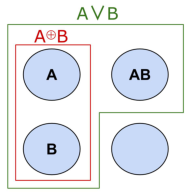
\includegraphics{figs/aorb-1} 

}

\caption[Inclusive disjunction (A$\vee$B) is true in situations where A, B, or both AB are true]{Inclusive disjunction (A$\vee$B) is true in situations where A, B, or both AB are true. Exclusive disjunction (A$\oplus$B) is true in situations where only A or only B is true.}\label{fig:aorb}
\end{figure}
\end{CodeChunk}

Given these complexities in the interpretation of disjunction, how can
children learn an underlyingly inclusive semantics for \emph{or}? A
previous investigation has suggested that children rarely hear the word
\emph{or}; and when they do, they hear the exclusive interpretation.
Morris (2008) investigated instances of \emph{and} and \emph{or} in
parents' and children's speech using 240 transcripts in the CHILDES
database (MacWhinney, 2000). He found that compared to \emph{and},
\emph{or} is extremely rare in child-directed speech and that children
start to produce \emph{and} earlier than \emph{or}. He showed that for
\emph{and}, children matched their parents' level of production at age
3, while for \emph{or}, they did not have comparable frequencies to
their parents even at age 5. Furthermore, the majority of \emph{or}
examples children heard (75-80\%) and produced (90\%) had exclusive
interpretations. Based on these findings, he concluded that children's
early meaning for \emph{or} is exclusive disjunction and that they learn
the inclusive meaning in later stages of development (possibly at age 6
or 7).

Contrary to Morris (2008)'s conclusion, a series of experimental studies
found that children between the ages of 3 and 5 interpret \emph{or} as
inclusive disjunction (Chierchia, Crain, Guasti, Gualmini, \& Meroni,
2001; Crain, 2012; Jasbi \& Frank, 2016). Given Morris (2008)'s finding
that the majority of \emph{or} examples children hear are exclusive, how
can children learn to interpret \emph{or} as inclusive? Crain (2012)
considered it unlikely that children learn the meaning of \emph{or} from
the examples they hear in adult usage. Instead, he argued that children
rely on an innate knowledge that the meaning of a disjunction word must
be inclusive. In other words, upon hearing a connective word, children
consider inclusive disjunction (A \(\vee\) B) as a viable candidate for
its meaning but not exclusive disjunction (A \(\oplus\) B).

Here we present two studies, investigating the role of input in
children's acquisition of disjunction. In Study 1, we used a larger
corpus (9,097 transcripts in CHILDES) than that of Morris (2008) to
investigate the frequencies of \emph{and}/\emph{or} in parent-child
interactions. First we replicated Morris (2008)`s results. We found that
\emph{and} is at least 10 times more frequent than \emph{or} in
child-directed speech, and that children start producing \emph{and}
slightly earlier than \emph{or} on average. We also found that for
\emph{and}, children reach their parents' level of production around 3
years of age. For \emph{or}, however, children's production increased
between 2.5 and 4 years and stayed constant afterward, but it did not
reach parents' level. We argue that this may be due to an asymmetry in
the speech acts produced by parents and children. Overall, parents ask
more questions from children than vice versa. Since \emph{or} is more
frequent in questions than declaratives, children's lower production of
questions than parents may result in lower productions of \emph{or} as
well. We show that when we split children's productions by speech act,
children's production of \emph{or} in declaratives (but not questions)
is comparable to that of parents. In Study 2, we conducted an annotation
study to check the frequencies of \emph{or}'s exclusive and inclusive
interpretations as well as conceptual and prosodic cues that accompany
it. We replicated Morris (2008)'s finding that the majority of \emph{or}
examples in child-directed speech have an exclusive interpretation.
However, we also show that these exclusive interpretations correlate
systematically with conceptual and prosodic cues. Exclusive
interpretations were either conceptually inconsistent or carried a
distinct rise-fall intonation. We show that setting aside these cases,
the interpretation of a disjunction is most often inclusive. We build a
learning model that uses intonation and conceptual consistency to
predict the interpretation of a disjunction with high accuracy even
given relatively few examples. These results suggest that children can
rely on cues present in child-directed speech to tease apart the
exclusive vs.~inclusive interpretation of disjunction and map the
meaning of \emph{or} accordingly.

\section{Study 1: Corpus Study}\label{study-1-corpus-study}

First, we conducted a large-scale exploratory investigation of
\emph{and} and \emph{or} productions in parents' and children's speech.
The goal of the study was to find out when children start producing
these words and what is their frequency of usage.

\begin{CodeChunk}
\begin{figure}[tb]
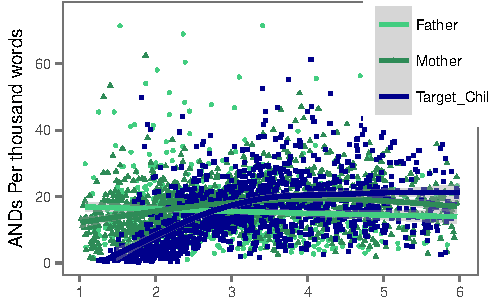
\includegraphics{figs/OverallConnectivePlots-1} \caption[Relative frequency of and/or in parents' (green) and children's (blue) speech between ages 1-6 years]{Relative frequency of and/or in parents' (green) and children's (blue) speech between ages 1-6 years.}\label{fig:OverallConnectivePlots}
\end{figure}
\end{CodeChunk}

\subsection{Methods}\label{methods}

\begin{CodeChunk}
\begin{figure*}[t]

{\centering 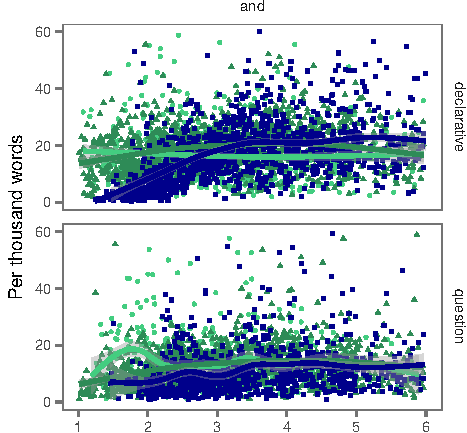
\includegraphics{figs/byspeechActPlots-1} 

}

\caption[Relative frequency of and/or in parents'/childern's speech between the ages of one and six years]{Relative frequency of and/or in parents'/childern's speech between the ages of one and six years.}\label{fig:byspeechActPlots}
\end{figure*}
\end{CodeChunk}

We accessed the Child Language Data Exchange System
(\href{https://childes.talkbank.org/}{CHILDES}; MacWhinney (2000)) via
the online platform \href{http://childes-db.stanford.edu/}{childes-db}
and its associated R package (Sanchez et al., in prep). We extracted all
instances of \emph{and} and \emph{or} in the English corpora (ENG-NA and
ENG-UK), with information on the child's age at the time of the
utterance as well as the utterance type. Utterances were coded as
``declarative'', ``question'', ``imperative'', or ``other'' according to
\href{https://talkbank.org/manuals/CHAT.html\#_Toc486414422}{the CHILDES
CHAT trascription format}. Since utterance types ``imperatives'' and
``other'' constituted a very small portion of utterances, we did not
include them in our analysis. We used utterance types as a proxy for
speech acts in this study (Austin, 1975). We limited our analysis to the
data between the ages 1 and 6 because there was limited data outside
this age range. We computed the relative frequency of connective
production by dividing the total number of \emph{and} and \emph{or}
tokens in the speech of fathers, mothers, and children at a particular
age by the total number of words spoken by them at that age. We present
the relative frequency as parts per thousand.

\subsection{Results}\label{results}

In Figure \ref{fig:OverallConnectivePlots}, we show the relative
frequencies of \emph{and} and \emph{or} in the speech of parents and
children between the ages of 1 and 6 years. In the speech of parents,
\emph{and} was produced around 20 times per thousand words, while
\emph{or} was only produced around 2 times per thousand words. These
results confirm previous findings that \emph{or} is much less frequent
than \emph{and} in child directed speech.

\begin{CodeChunk}
\begin{figure}[tb]
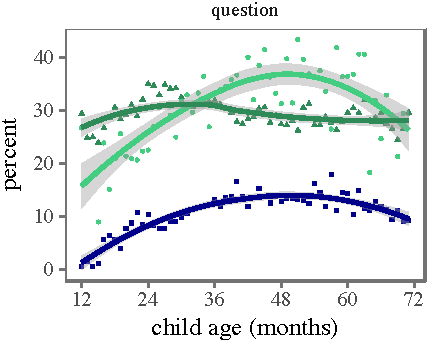
\includegraphics{figs/utteranceTypeByAgePlot-1} \caption[Proportion of questions (vs]{Proportion of questions (vs. declaratives) in child-parent interactions by age.}\label{fig:utteranceTypeByAgePlot}
\end{figure}
\end{CodeChunk}

The relative frequencies of \emph{and} and \emph{or} in children's
speech show different developmental trajectories. The production of
\emph{and} starts between 12-18 months (1-1.5 years) and increases until
it reaches parents' level around 30 months (2.5 years). The production
of \emph{or}, on the other hand, starts slightly later between 18-30
months (1.5-2.5 years). It increases between 30-42 months (2.5-3.5
years) and stays at a constant rate -- one \emph{or} per thousand words
-- between 42-72 months (3.5-6 years). These results replicate Morris
(2008)`s findings that \emph{or} is produced later than \emph{and}, and
that it reaches parents' rate of production later as well. While Morris
(2008) discusses input frequency and conceptual complexity as possible
reasons for the differences in children's production of
\emph{and}/\emph{or}, we here consider the role of speech acts. Similar
to Morris (2008), we found most examples of \emph{and} in declaratives
(71\%) while examples of \emph{or} were as common in declaratives and
questions (46\% vs.~48\%). In addition, children produced fewer
questions than parents and increased their productions as they aged, but
they never reached parents' level (Figure
\ref{fig:utteranceTypeByAgePlot}). These results suggest that the
production of \emph{or} in children may be affected by the frequency and
the developmental trend of questions in children's speech.

We therefore computed the relative frequency of \emph{and}/\emph{or}
across questions and declaratives separately. Relative frequency was
computed as \emph{freq(target) / total--tokens}, where both are computed
within the utterances of a particular speaker (father, mother, child) in
a particular speech act (questions, declaratives). Overall, we found
that the relative frequency of \emph{and} is higher in declaratives than
in questions (18.75 vs.~12.27 words per thousand). The relative
frequency of \emph{or}, however, is higher in questions (0.9 vs.~2.2
words per thousand). Figure \ref{fig:byspeechActPlots} shows the
developmental trend of these relative frequencies, split by speech act.
Adults and children show close levels of productions for both
connectives in decleratives and for \emph{and} in questions. However,
children show a slow increase in the production of \emph{or} in
questions which was only close to parents' level at age 6. These results
suggest that children's lower overall production of \emph{or} may be
mostly due to their lower rate of asking questions from parents.
Overall, the study shows that children's productions are consistent with
an adult-like comprehension of \emph{and}/\emph{or} around the age four,
as some comprehension studies suggest (Crain, 2012; Jasbi \& Frank,
2016)

\section{Study 2: Annotation Study}\label{study-2-annotation-study}

Study 1 showed that even though \emph{or} is not frequent in
child-directed speech, children can produce it by the age 4. In Study 2,
we conducted an annotation study of \emph{or} productions in
child-directed speech. The goal of this study was to discover features
of child-directed speech that may help the acquisition of \emph{or}'s
meaning from infrequent data.

\subsection{Methods}\label{methods-1}

\begin{table}[b]
\centering
\begin{tabular}{lll}
 Category & Subcategory & Examples \\ 
  \hline
Interpretation & Exclusive & Wanna stay or go? \\ 
   & Inclusive & Anything to eat or drink? \\ 
   \hline
Intonation & Flat & I'll get tea or coffee. \\ 
   & Rise & Anything to eat or drink? \\ 
   & Rise-Fall & Wanna stay or go? \\ 
   \hline
Consistency & Consistent & I'll get tea or coffee. \\ 
   & Inconsistent & Wanna stay or go? \\ 
  \end{tabular}
\caption{Annotation categories and examples.} 
\end{table}

\begin{CodeChunk}
\begin{figure}[b]

{\centering 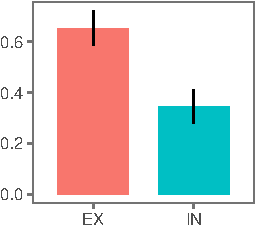
\includegraphics{figs/interpretation-1} 

}

\caption[Proportion of exclusive and inclusive interpretations of disjunction in child-directed speech]{Proportion of exclusive and inclusive interpretations of disjunction in child-directed speech. Error bars represent bootstrapped 95\% confidence intervals.}\label{fig:interpretation}
\end{figure}
\end{CodeChunk}

We accessed
\href{https://phonbank.talkbank.org/browser/index.php?url=Eng-NA/Providence/}{the
Providence corpus} (Demuth, Culbertson, \& Alter, 2006) via the phonbank
section of \href{https://talkbank.org/}{the TalkBank system}. We
extracted all instances of \emph{or} along with the two utterances
before and after to provide context using
\href{http://alpha.talkbank.org/clan/}{the CLAN software}. We annotated
the examples for three major categories: disjunction interpretation,
intonation, and conceptual consistency. Table 1 shows these categories
along with their subcategories and an example for each subcategory.

\subsubsection{Disjunction
Interpretation}\label{disjunction-interpretation}

This category was our dependent measure. Annotators listened to a
disjunction like ``A or B'' and decided whether the speaker intended to
imply ``A or B but not both'' (exclusive disjunction) or ``A or B, and
possibly both (inclusive disjunction).

\subsubsection{Intonation}\label{intonation}

For this category annotators listened to the utterances containing
disjunction and decided whether the intonation contour on the
disjunction is rise-fall, rise, or flat. Table 1 includes examples that
are prototypically read aloud with the intonation contour they are
subcategorized as.

\subsubsection{Consistency}\label{consistency}

For conceptual consistency, annotators decided whether the propositions
that make up the disjunction are inconsistent. Our annotators used the
following diagnostic to decide the consistency of the disjuncts: Two
disjuncts were marked as inconsistent if replacing the word \emph{or}
with \emph{and} produced a contradiction. For example, changing ``the
ball is in my room or your room'' to ``the ball is in my room and your
room'' produces a contradiction because the propositions cannot be both
true at the same time.

It is important to note here that this criterion is quite strict. In
many cases, the possibility of both propositions being true is ruled out
based on prior knowledge and expectations of the situation. For example,
when asking people whether they would like tea or coffee, it is often
assumed and expected that people choose one or the other. However,
wanting to drink both tea and coffee is not conceptually inconsistent.
It is just very unlikely. Our annotations of consistency are very
conservative in that they consider such unlikely cases as consistent. In
future research, relaxing this definition to allow for exclusion based
on prior expectations may allow us to capture more exclusive
interpretations of disjunction.

Finally, to test inter-rater reliability, the two raters annotated the
same 240 instances of disjunction. The inter-rater reliability was
calculated over 8 iterations of 30 examples each. Training only
completed after 3 consecutive iterations had substantial agreement
between the raters (Cohen's \(\kappa > 0.7\)) for all categories.

\begin{CodeChunk}
\begin{figure}[t]

{\centering 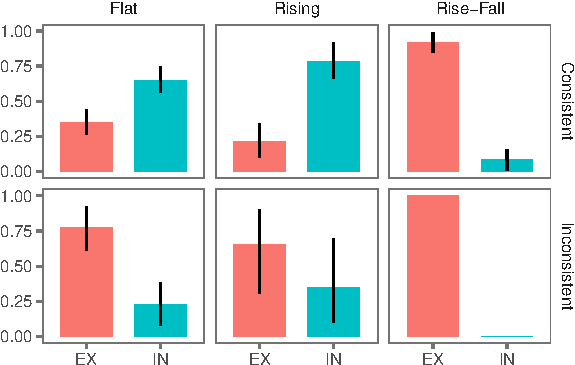
\includegraphics{figs/interpretationByIntonationAndConsistency-1} 

}

\caption[Exclusive and inclusive interpretations broken down by intonation (flat, rise, rise-fall) and consistency]{Exclusive and inclusive interpretations broken down by intonation (flat, rise, rise-fall) and consistency. Error bars represent bootstrapped 95\% confidence intervals.}\label{fig:interpretationByIntonationAndConsistency}
\end{figure}
\end{CodeChunk}

\subsection{Results}\label{results-1}

First, similar to Morris (2008), we found that the majority of \emph{or}
examples in CDS receive an exclusive interpretation (\(\sim\)\%65).
Figure \ref{fig:interpretation} shows this difference in distribution.
However, the rate of exclusive interpretations change systematically
when we break the data down by intonation and consistency (Figure
\ref{fig:interpretationByIntonationAndConsistency}). Given a rise-fall
intonation contour, a disjunction is almost always interpreted as
exclusive. Similarly, if the propositions are inconsistent, the
disjunction is most likely interpreted as exclusive. When either of
these two features are absent, a disjunction is more likely to receive
an inclusive interpretation.

We fit a mixed-effects binomial logistic regression using the package
\{lme4\} (Bates, Maechler, Bolker, Walker, \& others, 2014) in R with
fixed effects of intonation and consistency as well as random intercepts
for children. Both intonation and consistency were significant
predictors of exclusivity. Disjunctions were more likely to be
interpreted as exclusive if they received a rise-fall intonation
(\(\beta\)=-3.75, \(z\)=-8.49, \(p < 0.001\)) or if they were
inconsistent (\(\beta\)=-2.17, \(z\)=-8, \(p < 0.001\)). Disjunctions
were more likely to be interpreted as inclusive if they were consistent
and received a rising (\(\beta\)=0.67, \(z\)=2.44, \(p < 0.001\)) or
flat intonation (\(\beta\)=0.71, \(z\)=3.44, \(p < 0.001\)).

\begin{CodeChunk}
\begin{figure}[tb]

{\centering 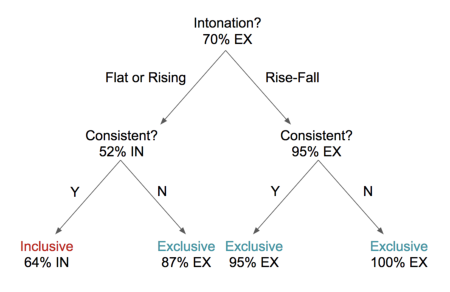
\includegraphics{figs/treeDiagram-1} 

}

\caption[Optimal decision tree training on 100 datapoints]{Optimal decision tree training on 100 datapoints. Provides series of two binary decisions to decide exlcusivity interpretation. Intonation $>$ 1.5 are rise-fall while intonation $<$ 1.5 are flat or rising. Consistency $>$ 0.5 are consistent while consistency $<$ 0.5 are  inconsistent.}\label{fig:treeDiagram}
\end{figure}
\end{CodeChunk}

\subsubsection{Classification Model}\label{classification-model}

The preceding analysis suggests that intonation and consistency are
related to the interpretation of disjunction. To investigate how
informative these patterns were more quantitatively, we built a model to
predict the interpretation of a disjunction after training on examples
annotated for intonation and consistency. To more easily understand the
rules governing exclusivity, we fit a decision tree model using Sci-kit
Learn's Decision Tree Module (Pedregosa et al., 2011). We randomly
sampled 100 examples for training and 300 examples for testing. Averaged
over 100 trials, the average accuracy of a binary tree was 83\%. More
remarkably, the tree achieved an average of 80\% accuracy after training
on only 20 examples (Figure \ref{fig:learningCurve}). The control flow
of the average decision tree on a single example is as follows. If
\emph{or} has neither rise-fall nor inconsistent disjuncts, it is marked
inclusive. Otherwise, exclusive (Figure \ref{fig:treeDiagram}). The
success of such a simple decision-tree indicates that children could use
a simple model to rapidly learn the exclusive interpretation of
\emph{or} from infrequent data.

\begin{CodeChunk}
\begin{figure}[tb]

{\centering 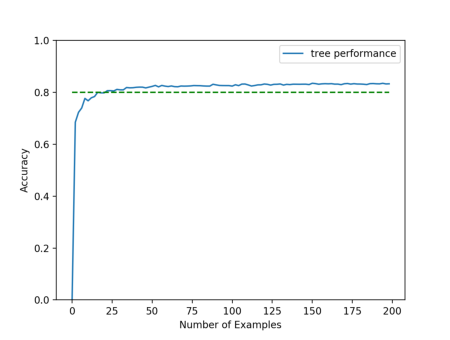
\includegraphics{figs/learningCurve-1} 

}

\caption[Decision Tree Accuracy as a function of number of examples seen]{Decision Tree Accuracy as a function of number of examples seen. Tested on a constant 300 examples. Dashed line marks 80\% accuracy threshold.}\label{fig:learningCurve}
\end{figure}
\end{CodeChunk}

\subsection{Summary}\label{summary}

In Study 2, we confirm Morris (2008)'s finding that exclusive
interpretations of \emph{or} are far more common than inclusive
interpretations. However, we also show that the majority of these
exclusive interpretations coincide with systematic indicators.
Disjunctions that are accompanied by rise-fall intonation or
inconsistent disjuncts are far more likely to be exclusive. Disjunctions
that do not bear these features are more likely to be inclusive.
Accounting for these external factors, a simple decision tree can
rapidly learn to predict the exclusive interpretation of the
disjunction.

\section{General Discussion}\label{general-discussion}

We addressed two puzzles in children's acquisition of disjunction.
First, previous comprehension and production studies provided different
accounts for the acquisition of \emph{and} and \emph{or}. Comprehension
studies suggested that children learn the meaning of both \emph{and} and
\emph{or} early and show an adult-like understanding of them by the age
4. However, production studies suggested that \emph{and} reaches the
parents' rate of production by the age 3 while \emph{or} does not even
at age 5. Study 1 showed that when we control for parent's and
children's production of speech acts, children around age 4 produce
\emph{and}/\emph{or} with relative frequencies comparable to those of
their parents. This observation unifies the picture from comprehension
and production studies: Children's acquisition of \emph{and} and
\emph{or} appears to take place between the ages of 2 and 4.

The second puzzle that this paper addressed was the problem of learning
an inclusive semantics for \emph{or} from the majority exclusive
instances in children's input. Previous studies showed that most
\emph{or} examples children hear receive an exclusive interpretation,
yet in comprehension tasks they interpret \emph{or} as inclusive. We
suggest that other independent cues in the input may allow children to
solve this problem. In Study 2, we replicated the pattern that most
interpretations of \emph{or} were exclusive. But most of these exclusive
interpretations were either constituted of two conceptually inconsistent
disjuncts or accompanied by a distinctive rise-fall intonation.
Disjunctions that did not show either of these two cues were typically
inclusive. If children track these cues, then they could tease apart the
semantic contribution of \emph{or} from the interpretive contribution of
the cues that accompany it.

We implemented this cue-based account in a decision-tree model, which
learned to predict the interpretation of a disjunction with high
accuracy after observing only a few examples. This model describes the
statistical properties of the data available to children, rather than
describing their learning process. Nevertheless, the success of this
model suggests that the systematicity of children's linguistic input
might allow them to decide correctly between exclusive and inclusive
semantics for disjunction. Such a learning account would obviate the
need for a principle that directly blocks exclusive disjunction as a
possible connective meaning. \emph{or} may not be assigned an exclusive
meaning simply because such a mapping is not supported by the language
children hear.

The findings here do not bear on other components of the logical
nativist account. A learning account still needs to address whether
candidate semantic representations -- inclusive and exclusive \emph{or},
as well as candidates for other connectives -- are innate or discovered
during development. Moreover, while conceptual consistency is likely a
reliable cue cross-linguistically, intonation may be a more
language-dependent cue and should be investigated further. Other
pragmatic and contextual effects that we did not examine might also bear
on children's interpretation of disjunction, and we expect that
exclusive interpretations not captured by our model might be captured by
these factors.

Form-meaning mapping in child language acquisition is often construed as
the task of associating a novel, isolated form such as \emph{gavagai} to
a well-delimited concept such as rabbit. The case of disjunction is more
complicated. \emph{or} cannot be isolated from either the conceptual
properties of the words and phrases that it combines with or the
prosodic contour of the utterance as a whole. Learning \emph{or} and
other function words requires a fuller consideration of the formal and
conceptual contexts in which they occur; our models must take these into
account.

\vspace{1em}
\fbox{\parbox[b][][c]{7.3cm}{\centering The data and code for this paper are available at\ \url{https://github.com/jasbi/JasbiJaggiFrank_cogsci2018}}}
\vspace{1em}

\section{Acknowledgements}\label{acknowledgements}

We would like to thank Eve V. Clark for her comments and guidance with
this project. We would also like to thank Kutay Serova and Salma Sebt.
This work was supported by NSF grant \#1456077, a Jacobs Foundation
Fellowship to MCF, and the Stanford Graduate Fellowship.

\section{References}\label{references}

\setlength{\parindent}{-0.1in} \setlength{\leftskip}{0.125in} \noindent

\hypertarget{refs}{}
\hypertarget{ref-austin1975things}{}
Austin, J. L. (1975). \emph{How to do things with words}. Oxford
university press.

\hypertarget{ref-bates2014lme4}{}
Bates, D., Maechler, M., Bolker, B., Walker, S., \& others. (2014).
Lme4: Linear mixed-effects models using eigen and s4. \emph{R Package
Version}, \emph{1}(7), 1--23.

\hypertarget{ref-chierchia2001acquisition}{}
Chierchia, G., Crain, S., Guasti, M. T., Gualmini, A., \& Meroni, L.
(2001). The acquisition of disjunction: Evidence for a grammatical view
of scalar implicatures. In \emph{Proceedings of the 25th boston
university conference on language development} (pp. 157--168).
Cascadilla Press Somerville, MA.

\hypertarget{ref-clark1995lexicon}{}
Clark, E. V. (1995). \emph{The lexicon in acquisition} (Vol. 65).
Cambridge University Press.

\hypertarget{ref-crain2012emergence}{}
Crain, S. (2012). \emph{The emergence of meaning}. Cambridge University
Press.

\hypertarget{ref-demuth2006word}{}
Demuth, K., Culbertson, J., \& Alter, J. (2006). Word-minimality,
epenthesis and coda licensing in the early acquisition of english.
\emph{Language and Speech}, \emph{49}(2), 137--173.

\hypertarget{ref-geurts2006exclusive}{}
Geurts, B. (2006). Exclusive disjunction without implicatures.
\emph{Ms., University of Nijmegen}.

\hypertarget{ref-grice1975logicconvo}{}
Grice, H. P. (1975). Logic and conversation. In P. Cole \& J. Morgan
(Eds.), \emph{Syntax and semantics} (Vol. 3: Speech Acts, pp. 43--58).
Academic Press.

\hypertarget{ref-jasbi2016cogsci}{}
Jasbi, M., \& Frank, M. C. (2016). \emph{The semantics and pragmatics of
logical connectives: Adults' and children's interpretations of and and
or in a guessing game}. Proceedings of the 39th Annual Conference of the
Cognitive Science Society.

\hypertarget{ref-macwhinney2000childes}{}
MacWhinney, B. (2000). \emph{The childes project: The database} (Vol.
2). Psychology Press.

\hypertarget{ref-morris2008logically}{}
Morris, B. J. (2008). Logically speaking: Evidence for item-based
acquisition of the connectives and \&amp; or. \emph{Journal of Cognition
and Development}, \emph{9}(1), 67--88.

\hypertarget{ref-pedregosa2011scikit}{}
Pedregosa, F., Varoquaux, G., Gramfort, A., Michel, V., Thirion, B.,
Grisel, O., \ldots{} others. (2011). Scikit-learn: Machine learning in
python. \emph{Journal of Machine Learning Research}, \emph{12}(Oct),
2825--2830.

\hypertarget{ref-pruitt2013interpretation}{}
Pruitt, K., \& Roelofsen, F. (2013). The interpretation of prosody in
disjunctive questions. \emph{Linguistic Inquiry}, \emph{44}(4),
632--650.

\hypertarget{ref-childesdb}{}
Sanchez, A., Meylan, S., Braginsky, M., MacDonald, K., Yurovsky, D., \&
Frank, M. C. (in prep). Childes-db: A flexible and reproducible
interface to the child language data exchange system (childes).

\end{document}
